%% abtex2-modelo-trabalho-academico.tex, v-1.9.6 laurocesar
%% Copyright 2012-2016 by abnTeX2 group at http://www.abntex.net.br/ 
%%
%% This work may be distributed and/or modified under the
%% conditions of the LaTeX Project Public License, either version 1.3
%% of this license or (at your option) any later version.
%% The latest version of this license is in
%%   http://www.latex-project.org/lppl.txt
%% and version 1.3 or later is part of all distributions of LaTeX
%% version 2005/12/01 or later.
%%
%% This work has the LPPL maintenance status `maintained'.
%% 
%% The Current Maintainer of this work is the abnTeX2 team, led
%% by Lauro César Araujo. Further information are available on 
%% http://www.abntex.net.br/
%%
%% This work consists of the files abntex2-modelo-trabalho-academico.tex,
%% abntex2-modelo-include-comandos and abntex2-modelo-references.bib
%%

% ------------------------------------------------------------------------
% ------------------------------------------------------------------------
% abnTeX2: Modelo de Trabalho Academico (tese de doutorado, dissertacao de
% mestrado e trabalhos monograficos em geral) em conformidade com 
% ABNT NBR 14724:2011: Informacao e documentacao - Trabalhos academicos -
% Apresentacao
% ------------------------------------------------------------------------
% ------------------------------------------------------------------------

\documentclass[
	% -- opções da classe memoir --
	12pt,				% tamanho da fonte
	openright,			% capítulos começam em pág ímpar (insere página vazia caso preciso)
	twoside,			% para impressão em recto e verso. Oposto a oneside
	a4paper,			% tamanho do papel. 
	% -- opções da classe abntex2 --
	%chapter=TITLE,		% títulos de capítulos convertidos em letras maiúsculas
	%section=TITLE,		% títulos de seções convertidos em letras maiúsculas
	%subsection=TITLE,	% títulos de subseções convertidos em letras maiúsculas
	%subsubsection=TITLE,% títulos de subsubseções convertidos em letras maiúsculas
	% -- opções do pacote babel --
	english,			% idioma adicional para hifenização
	french,				% idioma adicional para hifenização
	spanish,			% idioma adicional para hifenização
	brazil				% o último idioma é o principal do documento
	]{abntex2}

% ---
% Pacotes básicos 
% ---
\usepackage{lmodern}			% Usa a fonte Latin Modern			
\usepackage[T1]{fontenc}		% Selecao de codigos de fonte.
\usepackage[utf8]{inputenc}		% Codificacao do documento (conversão automática dos acentos)
\usepackage{lastpage}			% Usado pela Ficha catalográfica
\usepackage{indentfirst}		% Indenta o primeiro parágrafo de cada seção.
\usepackage{color}				% Controle das cores
\usepackage{graphicx}			% Inclusão de gráficos
\usepackage{microtype} 			% para melhorias de justificação
% ---

% Pacotes adicionais, usados no anexo do modelo de folha de identificação
\usepackage{longtable}
\usepackage{multicol}
\usepackage{multirow}
\usepackage[table,xcdraw]{xcolor}
\usepackage{hyperref}
\usepackage{amsmath}
\usepackage{tikz}
\usepackage{diagbox}
\usepackage{mathdots}
\usepackage{yhmath}
\usepackage{cancel}
\usepackage{color}
\usepackage{array}
\usepackage{amssymb}
\usepackage{gensymb}
\usepackage{rotating}
\usepackage{siunitx}
\usepackage{float} % para utilizar o H de tabelas e figuras e mante-las no lugar
\usepackage{listings}
\usepackage{xcolor}
\usepackage{verbatim}
\usepackage{chngcntr}
\usepackage{svg}
\svgpath{{img/}}

\definecolor{codegreen}{rgb}{0,0.6,0}
\definecolor{codegray}{rgb}{0.5,0.5,0.5}
\definecolor{codepurple}{rgb}{0.58,0,0.82}
\definecolor{backcolour}{rgb}{0.95,0.95,0.92}

\lstdefinestyle{mystyle}{
    backgroundcolor=\color{backcolour},   
    commentstyle=\color{codegreen},
    keywordstyle=\color{magenta},
    numberstyle=\tiny\color{codegray},
    stringstyle=\color{codepurple},
    basicstyle=\ttfamily\footnotesize,
    breakatwhitespace=false,         
    breaklines=true,                 
    captionpos=t,                    
    keepspaces=true,                 
    numbers=left,                    
    numbersep=5pt,                  
    showspaces=false,                
    showstringspaces=false,
    showtabs=false,                  
    tabsize=2
}

\renewcommand{\lstlistingname}{Algoritmo}
\renewcommand{\lstlistlistingname}{Lista de \lstlistingname s}

\newcommand{\quotes}[1]{``#1''}


\lstset{style=mystyle}

% ---
% Pacotes de citações
% ---
\usepackage[brazilian,hyperpageref]{backref}	 % Paginas com as citações na bibl
\usepackage[alf]{abntex2cite}	% Citações padrão ABNT

% --- 
% CONFIGURAÇÕES DE PACOTES
% --- 

% ---
% Configurações do pacote backref
% Usado sem a opção hyperpageref de backref
\renewcommand{\backrefpagesname}{Citado na(s) página(s):~}
% Texto padrão antes do número das páginas
\renewcommand{\backref}{}
% Define os textos da citação
\renewcommand*{\backrefalt}[4]{
	\ifcase #1 %
		Nenhuma citação no texto.%
	\or
		Citado na página #2.%
	\else
		Citado #1 vezes nas páginas #2.%
	\fi}%
% ---

% ---
% Informações de dados para CAPA e FOLHA DE ROSTO
% ---
\titulo{Estudo Experimental de um Sistema de Comunicação LoRa para Aplicação em Satélites}
\autor{Lucas Saavedra Vaz}
\local{São José dos Campos}
\data{2022}
\orientador{Prof. Dr. Lauro Paulo da Silva Neto}
\coorientador{Prof. Dr. Arlindo Flávio da Conceição}
\instituicao{%
  Universidade Federal de São Paulo
  \par
  Instituto de Ciência e Tecnologia
  \par
  Bacharelado em Engenharia de Computação}
\tipotrabalho{Trabalho de Conclusão de Curso}
% O preambulo deve conter o tipo do trabalho, o objetivo, 
% o nome da instituição e a área de concentração 
\preambulo{Trabalho de Conclusão de Curso submetido à Universidade Federal de São Paulo como parte dos
requisitos necessários para a obtenção do Grau de Bacharel em Engenharia de Computação.
}
% ---


% ---
% Configurações de aparência do PDF final

% alterando o aspecto da cor azul
\definecolor{blue}{RGB}{41,5,195}

% informações do PDF
\makeatletter
\hypersetup{
     	%pagebackref=true,
		pdftitle={\@title}, 
		pdfauthor={\@author},
    	pdfsubject={\imprimirpreambulo},
	    pdfcreator={LaTeX with abnTeX2},
		pdfkeywords={abnt}{latex}{abntex}{abntex2}{trabalho acadêmico}, 
		colorlinks=true,       		% false: boxed links; true: colored links
    	linkcolor=blue,          	% color of internal links
    	citecolor=blue,        		% color of links to bibliography
    	filecolor=magenta,      		% color of file links
		urlcolor=blue,
		bookmarksdepth=4
}
\makeatother
% --- 

% --- 
% Espaçamentos entre linhas e parágrafos 
% --- 

% O tamanho do parágrafo é dado por:
\setlength{\parindent}{1.3cm}

% Controle do espaçamento entre um parágrafo e outro:
\setlength{\parskip}{0.2cm}  % tente também \onelineskip

% ---
% compila o indice
% ---
\makeindex
% ---

% ----
% Início do documento
% ----
\begin{document}

% Seleciona o idioma do documento (conforme pacotes do babel)
%\selectlanguage{english}
\selectlanguage{brazil}

% Retira espaço extra obsoleto entre as frases.
\frenchspacing 

\counterwithout{lstlisting}{chapter}
\counterwithout{equation}{chapter}


% ----------------------------------------------------------
% ELEMENTOS PRÉ-TEXTUAIS
% ----------------------------------------------------------
% \pretextual

% ---
% Capa
% ---
\imprimircapa
% ---

% ---
% Folha de rosto
% (o * indica que haverá a ficha bibliográfica)
% ---
\imprimirfolhaderosto*
% ---

% ---
% Inserir a ficha bibliografica
% ---

% Isto é um exemplo de Ficha Catalográfica, ou ``Dados internacionais de
% catalogação-na-publicação''. Você pode utilizar este modelo como referência. 
% Porém, provavelmente a biblioteca da sua universidade lhe fornecerá um PDF
% com a ficha catalográfica definitiva após a defesa do trabalho. Quando estiver
% com o documento, salve-o como PDF no diretório do seu projeto e substitua todo
% o conteúdo de implementação deste arquivo pelo comando abaixo:
%
% \begin{fichacatalografica}
%     \includepdf{fig_ficha_catalografica.pdf}
% \end{fichacatalografica}

\begin{fichacatalografica}
	\sffamily
	\vspace*{\fill}					% Posição vertical
	\begin{center}					% Minipage Centralizado
	\fbox{\begin{minipage}[c][8cm]{13.5cm}		% Largura
	\small
	\imprimirautor
	
	\hspace{0.5cm} \imprimirtitulo  / \imprimirautor. --
	\imprimirlocal, \imprimirdata-
	
	\hspace{0.5cm} \pageref{LastPage} p. : il. (algumas color.) ; 30 cm.\\
	
	\hspace{0.5cm} \imprimirorientadorRotulo~\imprimirorientador\\
	
	\hspace{0.5cm}
	\parbox[t]{\textwidth}{\imprimirtipotrabalho~--~\imprimirinstituicao,
	\imprimirdata.}\\
	
	\hspace{0.5cm}
		1. LoRa.
		2. Satélites.
		3. Comunicação.
		I. Prof. Dr. Lauro Paulo da Silva Neto.
		II. Universidade Federal de São Paulo.
		III. Instituto de Ciência e Tecnologia.
		IV. Estudo Experimental de um Sistema de Comunicação LoRa para Aplicação em Satélites. 			
	\end{minipage}}
	\end{center}
\end{fichacatalografica}
% ---

% ---
% Inserir folha de aprovação
% ---

% Isto é um exemplo de Folha de aprovação, elemento obrigatório da NBR
% 14724/2011 (seção 4.2.1.3). Você pode utilizar este modelo até a aprovação
% do trabalho. Após isso, substitua todo o conteúdo deste arquivo por uma
% imagem da página assinada pela banca com o comando abaixo:
%
% \includepdf{folhadeaprovacao_final.pdf}
%
\begin{folhadeaprovacao}

  \begin{center}
    {\ABNTEXchapterfont\large\imprimirautor}

    \vspace*{\fill}\vspace*{\fill}
    \begin{center}
      \ABNTEXchapterfont\bfseries\Large\imprimirtitulo
    \end{center}
    \vspace*{\fill}
    
    \hspace{.45\textwidth}
    \begin{minipage}{.5\textwidth}
        \imprimirpreambulo
    \end{minipage}%
    \vspace*{\fill}
   \end{center}
        
   Trabalho aprovado. \imprimirlocal, 23 de Janeiro de 2023:

   \assinatura{\textbf{\imprimirorientador} \\ Orientador} 
   \assinatura{\textbf{Professor} \\ Prof. Dr. Henrique Alves de Amorim}
   \assinatura{\textbf{Professor} \\ Prof. Dr. Sérgio Ronaldo Barros dos Santos}
   %\assinatura{\textbf{Professor} \\ Convidado 3}
   %\assinatura{\textbf{Professor} \\ Convidado 4}
      
   \begin{center}
    \vspace*{0.5cm}
    {\large\imprimirlocal}
    \par
    {\large\imprimirdata}
    \vspace*{1cm}
  \end{center}
  
\end{folhadeaprovacao}
% ---

% ---
% Dedicatória
% ---
\begin{dedicatoria}
   \vspace*{\fill}
   \centering
   \noindent
   \textit{Para minha mãe Nevinka e meu pai Renato} \vspace*{\fill}
\end{dedicatoria}
% ---

% ---
% Agradecimentos
% ---
\begin{agradecimentos}

O desenvolvimento deste trabalho de conclusão de curso contou com a ajuda de diversas pessoas, dentre as quais eu agradeço:

Aos professores orientadores, que durante meses me acompanharam pontualmente, dando todo o auxílio necessário para a elaboração do projeto.

Aos professores do curso de Engenharia de Computação e Ciência e Tecnologia que, através dos seus ensinamentos, permitiram que eu pudesse hoje estar concluindo este trabalho.

A minha família, que me incentivou a cada momento, não permitiu que eu desistisse e tornou este trajeto acadêmico possível.

Aos meus amigos, pelo companheirismo durante todos esses anos e pelo afastamento temporário.

\end{agradecimentos}
% ---

% ---
% Epígrafe
% ---
\begin{epigrafe}
    \vspace*{\fill}
	\begin{flushright}
		\textit{\quotes{A ciência não é sobre o porquê! É sobre o porquê não!}} - Cave Johnson
	\end{flushright}
\end{epigrafe}
% ---

% ---
% RESUMOS
% ---

% resumo em português
\setlength{\absparsep}{18pt} % ajusta o espaçamento dos parágrafos do resumo
\begin{resumo}

Os nanossatélites para orbitas baixas estão cada vez mais populares devido a seu baixo custo, baixa complexidade e a capacidade de realização de experimentos espaciais com maior independência. Além disso, lançamentos de satélites de pequeno porte podem ter seu preço reduzido com o compartilhamento do compartimento de carga de foguetes (\emph{rideshare}), assim tornando essa categoria muito atraente para uma grande parte de projetos sendo realizados (como por exemplo o satélite \quotes{Norby}). Uma das técnicas de modulação mais promissoras para este tipo de satélite é a tecnologia LoRa. Ela consiste em uma tecnologia de rádio por espalhamento de espectro em \emph{chirps}, que possibilita a transmissão de informações por longas distâncias ao mesmo tempo que requer baixa potência. Neste trabalho, é desenvolvido e estudado um subsistema de comunicação de pequenos satélites para testes de diferentes configurações da comunicação LoRa. São realizados testes para medir o desempenho em distância e taxa de sucesso da comunicação e demonstrar que diversas combinações de parâmetros são viáveis para a aplicação em satélites. Uma tabela com optimizações de parâmetros para diferentes requisitos de projeto é sintetizada ao final dos resultados.

 \textbf{Palavras-chave}: LoRa. Satélites. Comunicação.
\end{resumo}

% resumo em inglês
\begin{resumo}[Abstract]
 \begin{otherlanguage*}{english}
Nanosatellites for low orbits are increasingly popular due to their low cost, low complexity and ability to perform space experiments with greater independence. In addition, small satellite launches can have its price reduced with the sharing of the rocket cargo bay (rideshare), thus making this category very attractive for a large number of projects being carried out (such as the “Norby” satellite). One of the most promising modulation techniques for this type of satellite is LoRa technology. It consists of a chirp spread-spectrum radio technology that makes it possible to transmit information over long distances while requiring low power. In this work, a small satellite communication subsystem is developed and studied for testing different configurations of LoRa communication. Tests are carried out to measure the performance in distance and success rate of the communication and to demonstrate that several combinations of parameters are viable for application in satellites. A table with parameter optimizations for different design requirements is summarized at the end of the results.

   \vspace{\onelineskip}
 
   \noindent 
   \textbf{Keywords}: LoRa. Satellites. Communication.
 \end{otherlanguage*}
\end{resumo}

% ---
% inserir lista de ilustrações
% ---
\pdfbookmark[0]{\listfigurename}{lof}
\listoffigures*
\cleardoublepage
% ---

% ---
% inserir lista de tabelas
% ---
\pdfbookmark[0]{\listtablename}{lot}
\listoftables*
\cleardoublepage
% ---

% ---
% inserir lista de abreviaturas e siglas
% ---
\begin{siglas}
  \item[SF] \emph{Spreading Factor}
  \item[CR] \emph{Coding Rate}
  \item[BW] \emph{Bandwidth}
  \item[ITU] \emph{International Telecommunication Union}
  \item[IEEE] \emph{Institute of Electrical and Electronics Engineers}
  \item[SOC] \emph{System-on-a-Chip}
  \item[LEO] \emph{Low Earth Orbit}
  \item[M2M] \emph{Machine to Machine}
  \item[IoT] \emph{Internet of Things}
  \item[LED] \emph{Light-Emitting Diode}
  \item[OLED] \emph{Organic Light-Emitting Diode}
  \item[RTOS] \emph{Real-Time Operating System}
\end{siglas}
% ---

% ---
% inserir lista de símbolos
% ---
\begin{simbolos}
  \item[$ \alpha $] Letra grega Alpha minúscula
  \item[$ \beta $] Letra grega Beta minúscula
  \item[$ \sigma $] Letra grega Sigma minúscula
  \item[$ \rho $] Letra grega Rho minúscula
\end{simbolos}
% ---

% ---
% inserir o sumario
% ---
\pdfbookmark[0]{\contentsname}{toc}
\tableofcontents*
\cleardoublepage
% ---



% ----------------------------------------------------------
% ELEMENTOS TEXTUAIS
% ----------------------------------------------------------
\textual

% ----------------------------------------------------------
\chapter{Introdução}
% ----------------------------------------------------------

Hoje em dia, os dispositivos de Internet das Coisas (IoT) são amplamente utilizados em todo o mundo onde uma rede de internet está disponível. No entanto, a cobertura global ainda não foi alcançada, particularmente nas montanhas, desertos, florestas e sobre o mar. Em vez disso, a comunicação via satélite é usada nessas regiões isoladas. A órbita baixa do planeta (LEO), que fica a menos de 1.000 km acima da Terra, é onde os satélites usados para a rede da Internet das Coisas são frequentemente lançados. A capacidade de enviar dados com menos atraso, perdas mínimas de potência de transmissão e uma frequência orbital mais alta são as principais vantagens dos satélites LEO. \cite{intro_2021}

Muitas empresas e organizações acadêmicas estão tentando lançar esses satélites nos últimos anos devido à tendência de uma pequena constelação de satélites LEO para aplicações IoT. Um tipo de satélite com maior potencial para essa aplicação é o CubeSat. Essa categoria de veículos espaciais permitem a criação de plataformas de experimento de baixo custo de desenvolvimento, lançamento e pequena escala de projeto. Além disso, estas plataformas têm um curto ciclo de desenvolvimento, podendo ser elaborado e lançado em apenas alguns meses \cite{heidt_2000}. Também é possível diminuir custos de projeto com o compartilhamento do compartimento de carga de um foguete entre vários nanossatélites (\emph{rideshare}).

Os sistemas de comunicação de rádio dos nanossatélites CubeSat geralmente usam diferentes variações de modulação de frequência ou fase.
No entanto, a eficiência do link de rádio pode ser consideravelmente aumentada utilizando técnicas de modulação mais avançadas.
Uma dessas técnicas é a modulação LoRa, amplamente utilizada em redes de sensores sem fio IoT para comunicação máquina-a-máquina (M2M). Os dispositivos IoT são frequentemente usados com satélites, apesar de não serem exclusivos. 
Essa abordagem de modulação usa um sinal \emph{chirp} de banda larga com uma frequência que aumenta ou diminui linearmente com o tempo para codificar os dados.

A alta velocidade de um satélite viajando sobre a estação terrestre cria um efeito Doppler significativo na frequência do sinal enviado no ponto de recepção, que é uma característica comum do link de rádio satélite-terra.
A abordagem de espalhamento espectral da modulação LoRa fornece uma baixa sensibilidade integrada ao efeito Doppler quando comparada a seus concorrentes \cite{doroshkin_2018}.

Com a popularização deste tipo de satélite e técnica de modulação, estudaremos neste trabalho a influência de cada parâmetro configurável da comunicação LoRa para a criação de um subsistema de comunicação em um nanossatélite. Neste trabalho, são revisados conceitos teóricos importantes das tecnologias utilizadas. Em seguida, é desenvolvida uma plataforma para a transmissão de rádio LoRa. Com isso são feitos testes com relação a distância e sucesso de transmissão para diferentes tipos de configurações, aos quais resultados são discutidos e analisados.

% ----------------------------------------------------------

\chapter{Objetivos}

\section{Objetivos Gerais}

Neste trabalho é proposto um ensaio experimental de um sistema da comunicação para nanossatélites utilizando a tecnologia LoRa para a transmissão de informações (e.g. Dados de sensores de temperatura, pressão e carga de bateria). As análises são focadas na implementação de técnicas em software e configurações para tornar a conexão mais confiável e eficiente.

\section{Objetivos Específicos}

\begin{itemize}
    \item Utilizar microcontroladores para testes de transmissões LoRa;
    \item Analisar e implementar as possíveis configurações de transmissão como, por exemplo, fator de espalhamento e largura de banda;
    \item Aplicar recursos de software para tornar a transmissão mais confiável;
    \item Produzir um \emph{framework} para selecionar diferentes parâmetros LoRa com base no requisito do projeto;
\end{itemize}

\begin{comment}

\section{Cronograma}

\begin{table}[H]
\centering
\caption{Cronograma das Atividades Desenvolvidas}
\label{tab:cronograma}
\begin{tabular}{|l|l|l|l|l|l|l|}
\hline
Atividade                       & Mês 1 & Mês 2 & Mês 3 & Mês 4 & Mês 5 & Mês 6 \\ \hline
Estudo da fundamentação teórica & X     &       &       &       &       &       \\ \hline
Desenvolvimento do algoritmo    &       & X     & X     &       &       &       \\ \hline
Testes simulados                &       &       &       & X     &       &       \\ \hline
Testes práticos                 &       &       &       &       & X     &       \\ \hline
Análise de resultados           &       &       &       &       &       & X     \\ \hline
Escrita da monografia           &       &       &       & X     & X     & X     \\ \hline
\end{tabular}
\end{table}

\end{comment}

% ----------------------------------------------------------

\chapter{Fundamentação Teórica}
% ----------------------------------------------------------

\section{Nanossatélites}

Em uma publicação de 1992 da Universidade de Surrey, a palavra \quotes{nanossatélite} apareceu pela primeira vez impressa. Apesar de terem sido inicialmente classificados como espaçonaves com massa inferior a 10 kg, os nanossatélites são agora mais especificamente definidos como espaçonaves com massa de 1 a 10 kg. O lançamento do Vanguard 1 pelos Estados Unidos em 1958, o primeiro nanossatélite em funcionamento, foi possível graças à eletrônica de estado sólido e células solares primitivas. Ele tinha dois transmissores de onda contínua que permitiam tanto a estação terrestre quanto o monitoramento satélite-a-satélite das temperaturas internas da espaçonave e da densidade eletrônica total integrada. Embora esteja sem transmitir informações desde 1964, este primeiro nanossatélite ainda está em órbita.

Os desenvolvimentos de microeletrônica/nanoeletrônica, células solares, sistemas microeletromecânicos (MEMS) e design auxiliado por computador (CAD) permitiram nanossatélites que registram imagens visíveis com resolução terrestre de 5m, bem como nanossatélites que usam medições de ocultação de rádio do sistema de posicionamento global para monitorar concentrações de elétrons ionosféricos, níveis de umidade troposférica/estratosférica e temperaturas \cite{carvalho_2020}.

Cada satélite ao longo das duas primeiras décadas da era espacial tinha um design único. Eram obras de arte criadas pelos engenheiros espaciais. Até o final da década de 1970, as conexões padrão de espaçonaves eram praticamente inexistentes. Os microssatélites apareceram pela primeira vez no início da década de 1980 e, para reduzir custos, usaram uma estratégia de design totalmente nova, concentrando-se em tecnologias já existentes e usando componentes de prateleira (COTS) adequadamente qualificados \cite{camps_2019}.

A massa dos satélites aumentou por muitos anos desde seu surgimento. No entanto, parece que a era dos satélites de grande porte se encerrou, exceto por algumas aplicações militares, astronômicas e de comunicação. A fim de reduzir a complexidade, a \quotes{filosofia de missão} de um satélite pequeno frequentemente combina um único objetivo de missão com uma estratégia de projeto de orçamento que tem custos rigorosos e limitações de cronograma.

Os professores Jordi Puig-Suari da Universidade Politécnica do Estado da Califórnia (CalPoly) e Bob Twiggs da Universidade de Stanford desenvolveram o chamado padrão CubeSat em 1999 para permitir que estudantes de pós-graduação desenvolvam, projetem, implementem, testem e operem no espaço uma espaçonave completa em um quantidade de tempo \quotes{razoável} (ou seja, a duração de seus estudos).

CubeSats são pequenos satélites que são múltiplos de 1U (onde 1U tem, atualmente, dimensões 10 cm x 10 cm x 10 cm e pesam menos de 1,33 kg) e têm todos os mesmos subsistemas fundamentais que os satélites de grande porte, mas usam componentes de prateleira (COTS) em sua implementação. Apenas as interfaces externas mecânicas, ou pertencentes ao implantador orbital, são definidas pelo \quotes{padrão} do CubeSat. Embora não fosse inicialmente planejado para ser um padrão, sua simplicidade rapidamente levou à sua adoção como um padrão \quotes{de facto}. Um exemplo de CubeSat 1U pode ser observado na \autoref{fig:cubesat}.

\begin{figure}[H]
	\caption{\label{fig:cubesat}PhoneSat 2.5}
	\begin{center}
	    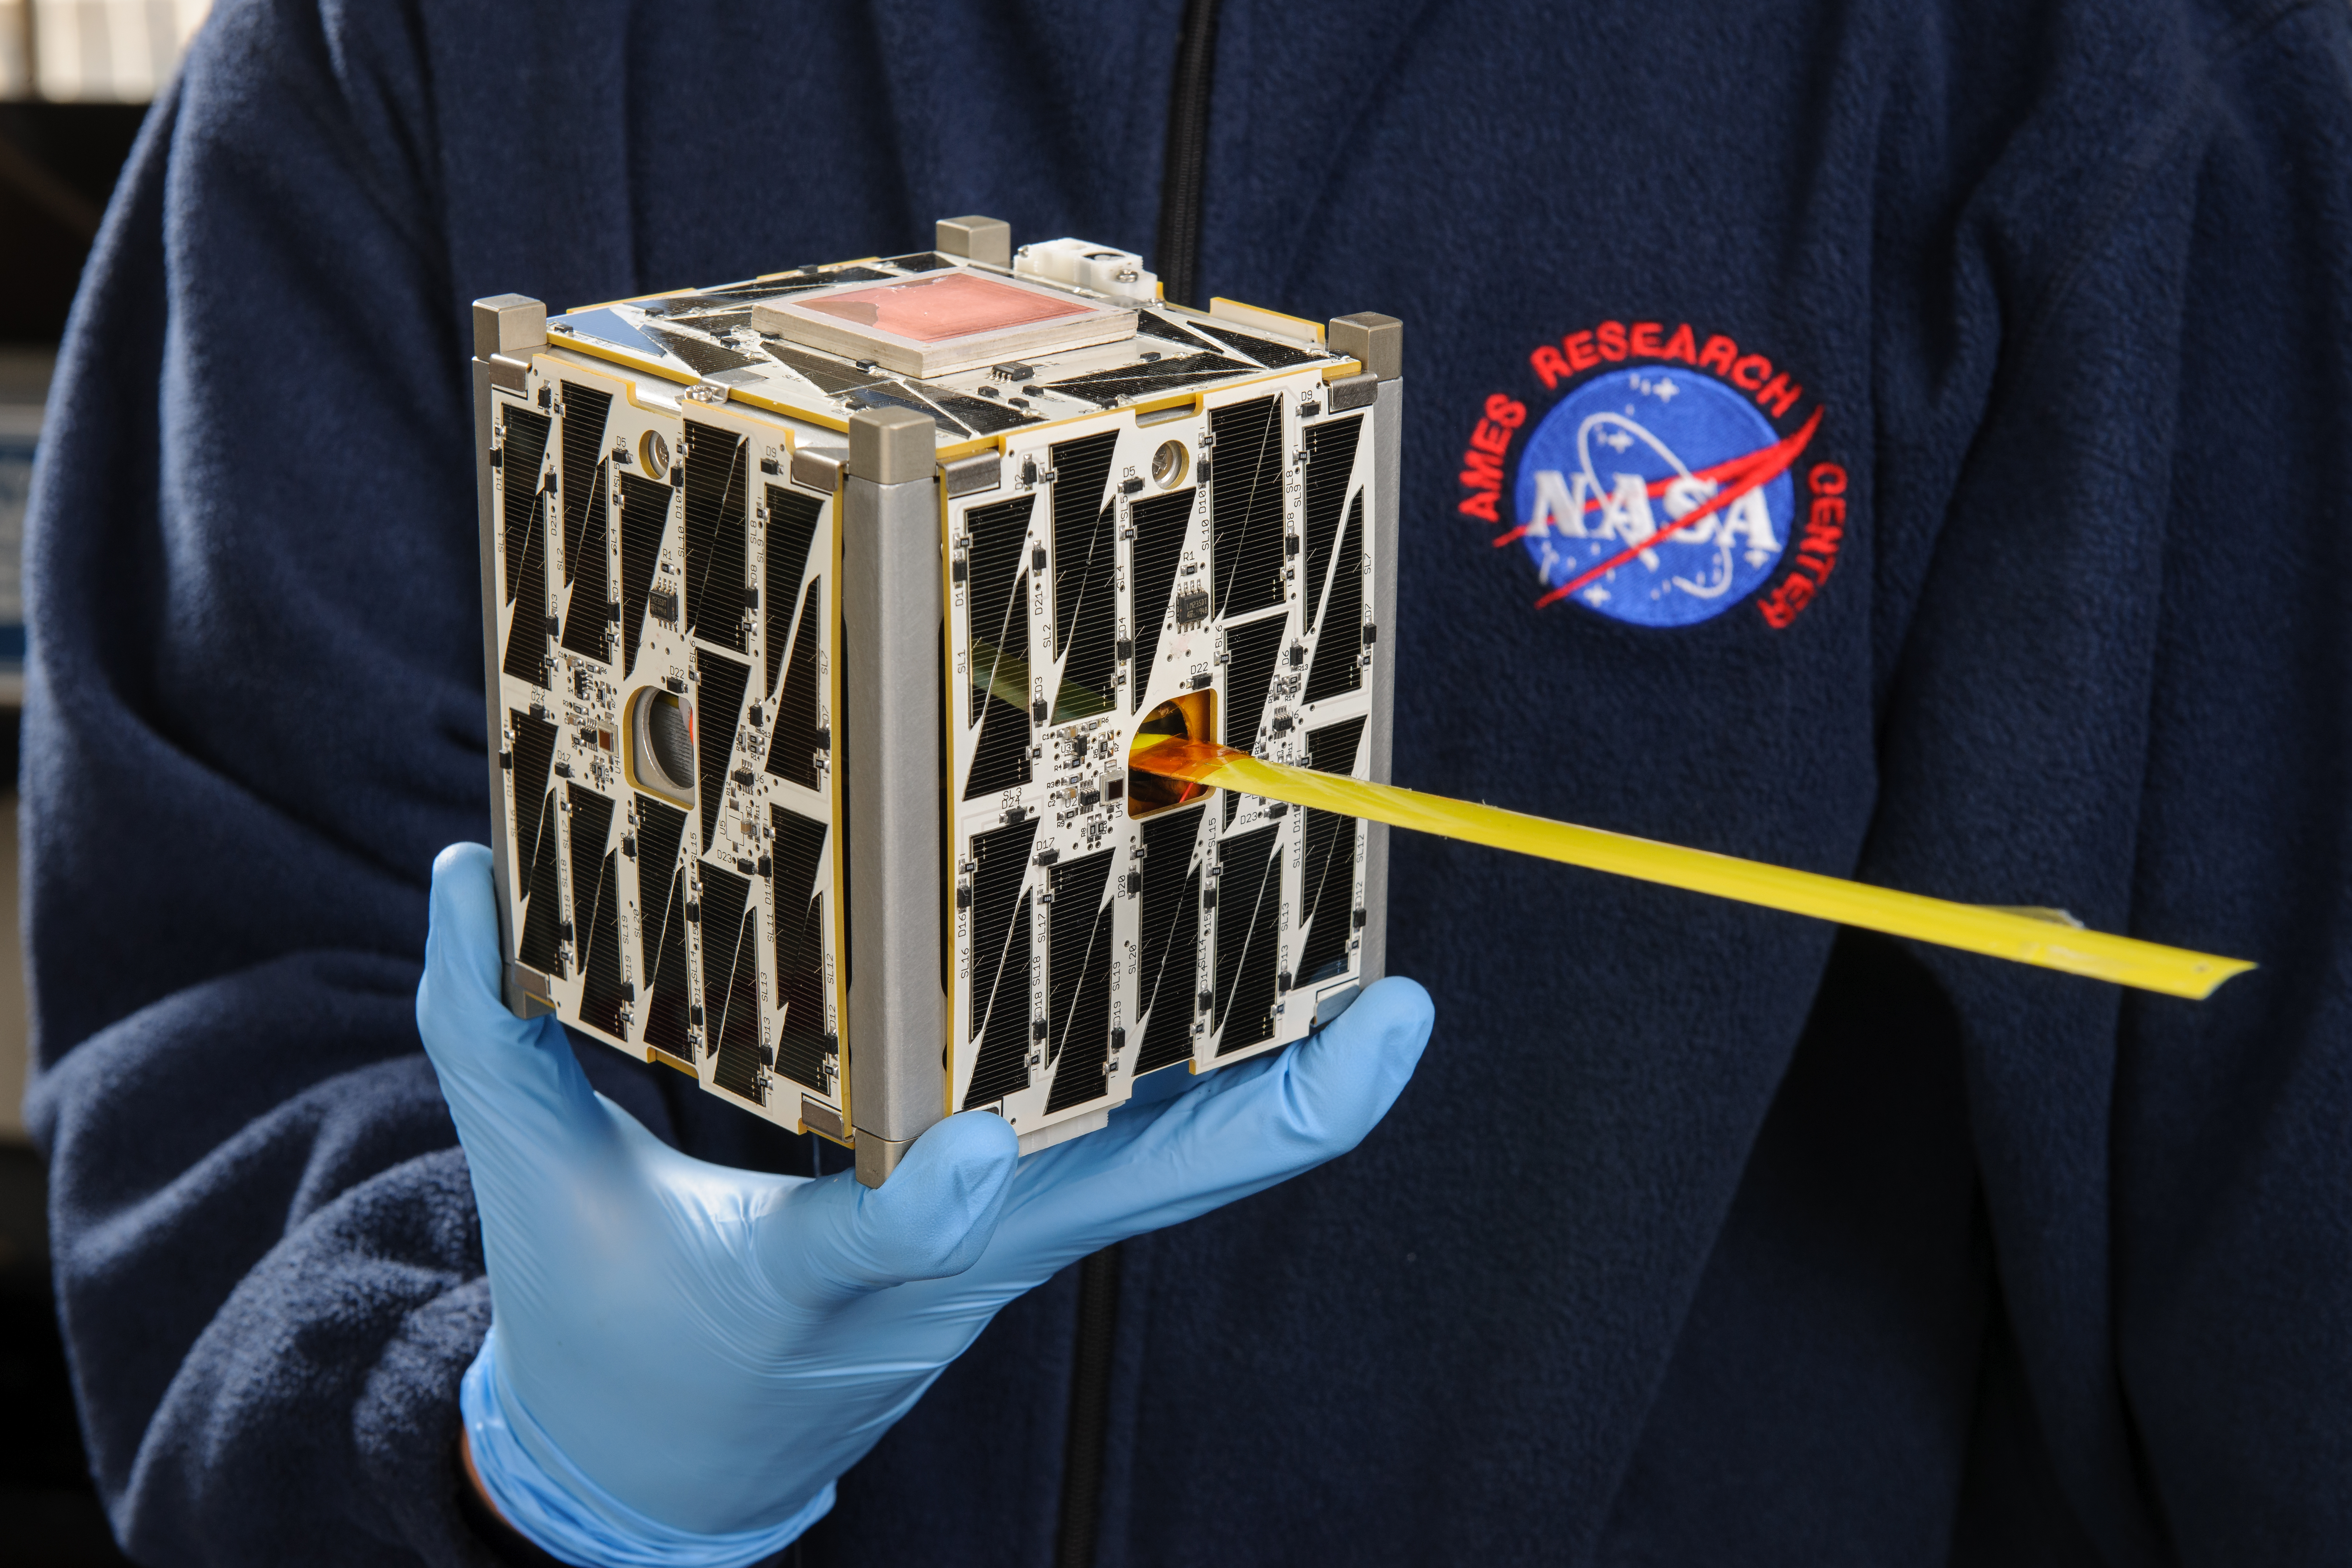
\includegraphics[scale=0.25]{img/Cubesat.jpg}
	\end{center}
	\legend{Fonte: \citeonline{thompson_2015}}
\end{figure}

A \autoref{fig:launches} exibe estatísticas históricas de nanossatélites ativos com massa entre 1 kg e 10 kg que foram lançados com sucesso e colocados em órbita de 1958 a 2017 (todos os CubeSats 1U estão incluídos). Revisões posteriores da Especificação do CubeSat elevaram a massa \quotes{U} para 1,33 kg do requisito original de 1 quilograma por \quotes{U} de volume. Além disso, vários CubeSats 1U iniciais estavam dentro de 10-20 g do objetivo original de 1000 g, indicando um déficit de massa de 2\% ou menos. Uma vez que todos os CubeSats \quotes{sub-U}, como PocketQubes e SunCubes, estão da faixa de massa dos picossatélites, eles não estão representados na \autoref{fig:launches} \cite{carvalho_2020}.

\begin{figure}[H]
	\caption{\label{fig:launches}Lançamentos de nanossatélites por ano}
	\begin{center}
	    \includegraphics[scale=0.4]{img/Launches.png}
	\end{center}
	\legend{Fonte: \citeonline[p. 2]{carvalho_2020}}
\end{figure}

\section{Sistemas Embarcados}

Utilizamos uma diversidade de dispositivos para facilitar as atividades a serem realizadas.
Esses dispositivos podem ser analógicos ou digitais e possuir algum processamento para o tratamento de dados. É fácil distinguir dispositivos que possuem processamento de dados ou não. Um exemplo de dispositivo sem processamento é o chuveiro pois não há nenhuma necessidade de tratamento lógico para o seu funcionamento. Apenas o acionamento manual da válvula de água. Todo controle e regulagem de temperatura é feito apenas pelo circuito elétrico analógico. 

Por outro lado, é necessário processamento em certos tipos de dispositivos. Para isso utilizamos sistemas embarcados. Segundo o livro \emph{Microcontroladores e Microprocessadores},
\quotes{Um sistema embarcado é um dispositivo eletrônico e computacional
capaz de controlar periféricos a partir da execução de um programa,
que não seja um computador. É projetado para realizar tarefas
bem particulares, com grande restrição de recursos, memória e
processamento} \cite{perim_2017}.

Nos tempos atuais, a maioria dos produtos tecnológicos que consumimos necessita de algum tipo de processamento de dados digitais, como por exemplo televisão, celular, roteadores, micro-ondas e outros. As principais maneiras de se realizar o controle desses aparelhos pode ser por microcontroladores, microprocessadores ou FPGAs.

Microprocessadores geralmente possuem uma maior capacidade de processamento e propósitos gerais para a utilização do usuário, dessa maneira se tornando mais complexo e aumentando seu custo. Eles são compostos pela CPU e diversos outros chips de suporte como por exemplo a MMU (\emph{Memory Management unit}). 

Já microcontroladores, possuem processamento reduzido e foram criados para servir um propósito único dentro de um sistema. Por exemplo, o aparelho de micro-ondas, onde se há um microcontrolador interno que faz o controle da entrada de dados pelo usuário (utilizando o teclado) e aciona os mecanismos internos, controlando o tempo para garantir o funcionamento correto do aparelho e o cozimento do alimento da maneira desejada. O diagrama de blocos de um exemplo de microcontrolador pode ser observado na \autoref{fig:MCU}.

\begin{figure}[H]
	\caption{\label{fig:MCU}Diagrama de blocos de um microcontrolador}
	\begin{center}
	    \includegraphics[scale=0.4]{img/MCU.png}
	\end{center}
	\legend{Fonte: \citeonline[p. 15]{perim_2017}}
\end{figure}

Por último, os FPGAs são sistemas de alto custo e complexos que sintetizam circuitos eletrônicos de maneira programável e portanto criam uma maior flexibilidade. 

A evolução dos microcontroladores nos trouxe revoluções na categoria SOC (\emph{System On Chip}) que, atualmente, são amplamente utilizados em diversos tipos de dispositivos, mais notavelmente em smartphones.

Em satélites, um sistema embarcado com microcontroladores pode ser utilizado para se obter a função de comunicação entre diferentes estações devido ao fato do funcionamento ser estático e não necessitar da flexibilidade que microprocessadores ou FPGAs trazem para o sistema.

\subsection{ESP32}

Um dos microcontroladores com melhor custo benefício é o ESP32 da Espressif Systems. Ele possuí dois núcleos de arquitetura Xtensa LX6 de 32-bits, Fabricados utilizando a tecnologia de \SI{40}{\nano\meter} da TSMC. Toda memória interna, externa e periféricos estão localizados ao longo do barramento de dados e/ou instruções destes núcleos. O mapeamento de endereços desses núcleos é simétrico e, portanto, podem utilizar o mesmo endereçamento para acessar uma certa região de memória \cite{esp_trm_2022}.

A arquitetura Xtensa permite a criação de sistemas com grande grau de extensibilidade, alta densidade de código, implementação otimizada para baixa potência, alta performance e baixo custo \cite{xtensa_isa_2022}.

Além disso, uma das principais características do chip é possuir Wi-Fi \SI{2,4}{\giga\hertz} e Bluetooth de baixa potência. Isso cria uma enorme versatilidade em sistemas embarcados de diversas aplicações e potências. A interface SPI ou I2C são necessárias para a comunicação com modems LoRa. Outras funcionalidades como, por exemplo, UART, I2C e SDIO também estão presentes, como observado no diagrama de blocos do processador na \autoref{fig:ESP32_bd}.

\begin{figure}[H]
	\caption{\label{fig:ESP32_bd}Diagrama de blocos de um ESP32}
	\begin{center}
	    \includegraphics[scale=0.5]{img/ESP32_BD.png}
	\end{center}
	\legend{Fonte: \citeonline[p. 12]{esp_ds_2022}}
\end{figure}

\section{Comunicação por Rádio}

Rádio é a transmissão de informações usando campos eletromagnéticos não guiados que se propagam em frequências entre 3 kHz e 300 GHz. O termo \emph{ondas de rádio} é mais geralmente usado para descrever campos eletromagnéticos que se propagam nessa faixa de frequência. Em um sistema de comunicação de rádio, um transmissor converte a informação na forma analógica (como voz) ou digital (como dados) em uma onda de rádio, que então viaja para um receptor onde o sinal representado pela onda de rádio é transformado de volta à sua forma original.

O rádio não é a única forma de radiação eletromagnética que pode ser usada para transmitir dados. Infravermelho (IR), óptico, ultravioleta (UV), raios X e raios $\gamma$ são outros elementos do espectro eletromagnético. A única distinção essencial entre essas ocorrências é a faixa de comprimento de onda associada, que está relacionada à frequência \cite{ellingson_2016}.

Os diferentes tipos de radiação eletromagnética se comportam de maneira bastante distintas em suas aplicações, dependendo do comprimento de onda em relação aos tamanhos das estruturas no ambiente em que se propagam e do tipo de meio utilizado para essa propagação. As ondas de rádio viajam de forma relativamente eficaz através do ar e da maioria dos materiais de construção, e são espalhadas em vez de absorvidas e dissipadas por estruturas maiores que um comprimento de onda. Em contraste, as radiações IR, óptica e UV tendem a se dissipar significativamente mais rapidamente à medida que se propagam pelo ar ou pelos materiais de construção. Embora esse problema não afete tanto os raios X e os raios $\gamma$, eles são muito desafiadores para produzir e capturar e representam um risco para a saúde humana. Portanto, embora a radiação eletromagnética possa ser usada para comunicação sem fio em qualquer um desses regimes, o rádio é particularmente prático, pois é simples de usar, tem boas propriedades de propagação e geralmente é seguro.

Isso não quer dizer que o rádio não tenha desvantagens em comparação com outros tipos de radiação eletromagnética. O mais crucial deles é que a largura de banda é bastante restrita. Isso ocorre por dois motivos: Primeiro, o alcance das frequências disponíveis é limitado. Embora 300 GHz possa parecer muito, todos os benefícios mencionados acima são mais perceptíveis na extremidade inferior do espectro, e é por isso que a grande maioria dos sistemas de rádio opera em frequências abaixo de 15 GHz. Em contraste, a faixa de frequência óptica é de cerca de 2 PHz de largura e um único canal de comunicação óptica normalmente tem uma largura de banda de pelo menos 15 GHz. 

Devido ao espectro limitado que está disponível em frequências de rádio, esquemas de modulação mais complexos são usados para maximizar a eficiência espectral, ou a taxa na qual a informação pode ser transmitida com sucesso em uma determinada largura de banda. Os rádios agora precisam atender a padrões de desempenho rigorosos, pois esses esquemas mais complexos exigem hardware mais eficiente. As regiões de frequência mais alta do espectro eletromagnético não requerem medidas comparáveis devido à relativa disponibilidade do espectro.

A região de rádio do espectro eletromagnético abrange oito ordens de magnitude em frequência (ou comprimento de onda), com uma ampla gama de características e aplicações. Como resultado, é vantajoso dividir ainda mais o espectro de rádio em bandas. O esquema da União Internacional de Telecomunicações (ITU), descrito na \autoref{tab:radio_itu}, é um método popular para designar e nomear as bandas. \emph{Very low frequency} (VLF), \emph{low frequency} (LF), \emph{medium frequency} (MF) e assim por diante são abreviações para essas frequências. Um método diferente de dividir o espectro é o adotado pelo Instituto de Engenheiros Elétricos e Eletrônicos (IEEE), o qual nomeia bandas conforme apresentado na \autoref{tab:radio_ieee}. Os nomes das bandas são essencialmente históricos em ambos os casos e não fornecem nenhuma informação técnica específica.

\begin{table}[H]
\centering
\caption{Designação de bandas ITU}
\label{tab:radio_itu}
\begin{tabular}{|l|l|l|} 
\hline
\textbf{Banda} & \textbf{Frequências} & \textbf{Comprimentos de Onda}  \\ 
\hline
EHF            & 30-300 GHz           & 10-1 mm                        \\
SHF            & 3-30 GHz             & 10-1 cm                        \\
UHF            & 300-3000 MHz         & 1-0.1 m                        \\
VHF            & 30-300 MHz           & 10-1 m                         \\
HF             & 3-30 MHz             & 100-10 m                       \\
MF             & 300-3000 kHz         & 1000-100 m                     \\
LF             & 30-300 kHz           & 10-1 km                        \\
VLF            & 3-30 kHz             & 100-10 km                      \\
\hline
\end{tabular}
\legend{Fonte: \citeonline[p. 44]{ellingson_2016}}
\end{table}

\begin{table}[H]
\centering
\caption{Designação de bandas IEEE}
\label{tab:radio_ieee}
\begin{tabular}{|l|l|l|} 
\hline
\textbf{Banda} & \textbf{Frequências} & \textbf{Comprimentos de Onda}  \\ 
\hline
W              & 75-110 GHz           & 0,4-0,273 cm                   \\
V              & 40-75 GHz            & 0,75-0,4 cm                    \\
Ka             & 27-40 GHz            & 1,111-0,75 cm                  \\
K              & 18-27 GHz            & 1,667-1,111 cm                 \\
Ku             & 12-18 GHz            & 2,5-1,667 cm                   \\
X              & 8-12 GHz             & 3,75-2,5 cm                    \\
C              & 4-8 GHz              & 7,5-3,75 cm                    \\
S              & 2-4 GHz              & 15-7,5 cm                      \\
L              & 1-2 GHz              & 30-15 cm                       \\
\hline
\end{tabular}
\legend{Fonte: \citeonline[p. 44]{ellingson_2016}}
\end{table}

\subsection{Princípios do Espalhamento de Espectro}

A \autoref{fig:modulation} ilustra como a fase da portadora do sinal do transmissor muda em um sistema \emph{Direct Sequence Spread Spectrum} (DSSS) de acordo com uma sequência de código. Os códigos de espalhamento (ou sequências de chip), que multiplexam o sinal de dados com um padrão de bits predefinido a uma taxa significativamente maior, resultam em um sinal \quotes{mais rápido} com componentes de frequência mais altos do que o sinal de dados original. Isso indica que a largura de banda do sinal original foi excedida pela largura de banda do sinal transmitido.

Os bits da sequência de codificação são chamados de chips na terminologia de RF (para distinguir entre os bits mais longos e não codificados do sinal de dados original). O sinal transmitido é multiplicado com uma duplicata exata do código de espalhamento usado no transmissor de RF quando chega ao receptor de RF, criando uma cópia do sinal de dados original.

O sinal de dados desejado é recuperado no receptor multiplicando-se novamente com uma réplica criada localmente da sequência de espalhamento. Conforme visto na \autoref{fig:demodulation}, o sinal de propagação é efetivamente comprimido no receptor durante esse processo de multiplicação para retornar à sua largura de banda original não espalhada. Deve-se enfatizar que, para recuperar as informações com precisão, o receptor deve utilizar a mesma sequência de chip ou código do transmissor.

\begin{figure}[H]
	\caption{\label{fig:modulation}Modulação DSSS}
	\begin{center}
	    \includegraphics[scale=0.45]{img/Mod.png}
	\end{center}
	\legend{Fonte: \citeonline[p. 7]{semtech_2015}}
\end{figure}

\begin{figure}[H]
	\caption{\label{fig:demodulation}Demodulação DSSS}
	\begin{center}
	    \includegraphics[scale=0.45]{img/Demod.png}
	\end{center}
	\legend{Fonte: \citeonline[p. 7]{semtech_2015}}
\end{figure}

A proporção \quotes{chips por bit}, também conhecida como ganho de processamento (Gp), que geralmente é expressa em decibéis, determina o grau de espalhamento da sequência direta.

O ganho do processo do receptor não apenas fornece ganho de processamento intrínseco para a transmissão desejada (o que permite ao receptor recuperar com precisão o sinal de dados mesmo quando o SNR do canal é um número negativo), mas também reduz os sinais de interferência. Estes são dispersos fora da largura de banda de informação pretendida e são simples de filtrar \cite{semtech_2015}.

Em aplicações envolvendo transferência de dados, o DSSS é frequentemente empregado. No entanto, existem dificuldades para dispositivos e redes de baixo custo ou com restrição de energia. Isso é especialmente problemático para dispositivos com fontes de energia limitadas que não podem estar \quotes{sempre ligadas} e devem sincronizar com frequência e rapidez.

\subsection{\emph{Chirp Spread Spectrum}}

Na década de 1940, o \emph{Chirp Spread Spectrum} foi criado para aplicações de radar. Tradicionalmente utilizado em aplicações militares e comunicações seguras, esta técnica de modulação encontrou uso crescente em uma variedade de aplicações de comunicação de dados nos últimos vinte anos devido a seus requisitos de potência de transmissão comparativamente baixos e resistência inerente contra mecanismos de degradação de canal, como multi-percurso, desvanecimento, Doppler e interferências de bloqueio em banda.

Para aplicações que exigem maior mobilidade e alcance do que é possível com a camada física OQPSK DSSS, uma camada CSS foi adotada pelo IEEE para o padrão 802.15.4 das redes LR-WPANs \cite{semtech_2015}.

\subsection{LoRa}
\label{chap:lora}

LoRa é um sistema patenteado de modulação de espectro espalhado desenvolvido na tecnologia \emph{Chirp Spread Spectrum} (CSS) existente que fornece uma compensação entre sensibilidade e taxa de transferência de dados enquanto opera em um canal de largura de banda fixa de 125 kHz ou 500 kHz (para canais de uplink) e 500 kHz (para canais de downlink). A visualização dos diferentes SFs utilizados pela tecnologia LoRa pode ser observada na \autoref{fig:chirp}.

\begin{figure}[H]
	\caption{\label{fig:chirp}Chirps da modulação LoRa}
	\begin{center}
	    \includegraphics[scale=0.45]{img/Chirp.jpg}
	\end{center}
	\legend{Fonte: \citeonline[p. 5]{kim_2019}}
\end{figure}

Além disso, o LoRa aproveita os fatores de espalhamento ortogonais. Ao fazer otimizações adaptativas dos níveis de energia e taxas de dados de cada nó final vinculado, a rede é capaz de prolongar a vida útil da bateria dos nós finais conectados. Por exemplo, quando é necessário muito pouca banda de link, um dispositivo final próximo a um gateway deve transmitir dados com um fator de espalhamento baixo. Um dispositivo final distanciado, por outro lado, exigirá um fator de espalhamento consideravelmente maior durante a transmissão. Um dispositivo final distanciado, por outro lado, exigirá um fator de espalhamento consideravelmente maior durante a transmissão. Embora a taxa de dados seja inevitavelmente reduzida, esse fator de espalhamento mais alto oferece maior ganho de processamento e maior sensibilidade de recepção.

LoRa é apenas uma implementação de camada física (PHY), conforme especificado pelo modelo de rede de sete camadas OSI (implementação na \autoref{fig:OSI}). Um transmissor de RF em um dispositivo IoT transmite ondas de rádio LoRa para um receptor de RF em um gateway e vice-versa, usando o ar como meio em vez de cabos \cite{semtech_2020}.

\begin{figure}[H]
	\caption{\label{fig:OSI}Aplicação do LoRa na camada PHY e LoraWAN na camada MAC}
	\begin{center}
	    \includegraphics[scale=0.45]{img/OSI.jpg}
	\end{center}
	\legend{Fonte: \citeonline[p. 4]{kim_2019}}
\end{figure}

A modulação LoRa da Semtech soluciona todas as desvantagens associadas aos sistemas DSSS, resultando em uma alternativa robusta de baixo custo e baixo consumo de energia às abordagens padrão de comunicação de espectro espalhado.

Um sinal \emph{chirp} que muda continuamente na frequência é produzido na modulação LoRa para espalhar o espectro. Os deslocamentos de tempo e frequência entre o transmissor e o receptor neste sistema são equivalentes, o que reduz significativamente a complexidade do projeto do receptor. A largura de banda de frequência desse chirp é igual à largura de banda espectral do sinal.

O sinal chirp é modulado com o sinal de dados desejado após ser fragmentado em uma taxa de dados mais alta. Além disso, o LoRa possui uma técnica de correção de erros configurável que reduz a redundância e aumenta a robustez do sinal transmitido \cite{semtech_2015}.

Podemos sintetizar as vantagens da tecnologia LoRa nos seguintes itens:

\begin{itemize}
    \item A modulação LoRa é escalável em termos de largura de banda e frequência. Ela pode ser aplicada a aplicações de sequência direta de banda larga, bem como a saltos de frequência de banda estreita. O LoRa pode ser facilmente modificado para qualquer modo de operação com apenas algumas pequenas modificações no registro de configuração, ao contrário dos métodos convencionais de modulação de banda estreita ou banda larga.
    \item Semelhante ao FSK, o LoRa usa um método de modulação de envelope constante, possibilitando a reutilização de estágios de PA de baixo custo, baixa potência e alta eficiência sem fazer nenhuma alteração. Além disso, em comparação com um orçamento de enlace FSK tradicional, a potência de saída do transmissor pode ser diminuída, mantendo o mesmo ou melhor link de conexão, graças ao ganho de processamento associado ao LoRa.
    \item Um sinal LoRa tem um produto BT alto (BT > 1) e é particularmente resistente a técnicas de interferência dentro e fora da banda devido à sua natureza assíncrona. Ele oferece excelente imunidade a mecanismos de interferência de AM pulsado devido ao período do símbolo LoRa poder ser mais longo do que a rajada típica de curta duração dos sistemas FHSS de salto rápido. Valores típicos de seletividade fora do canal do receptor de 90 dB e rejeição co-canal melhor que 20 dB podem ser obtidos. Isso contrasta com os valores normais de rejeição de co-canal de -6 dB para modulação FSK e 50 dB para rejeição de canal vizinho e alternativo.
    \item O LoRa é melhor usado em áreas urbanas e suburbanas, onde o multi-percurso e o desvanecimento são predominantes, pois o pulso chirp é bastante amplo e fornece imunidade a esses dois fenômenos.
    \item O pulso LoRa experimenta uma ligeira mudança de frequência devido ao deslocamento Doppler, que também adiciona uma mudança muito pequena no eixo de tempo do sinal de banda base. A necessidade de fontes de clock de referência com precisão estrita é diminuída por essa tolerância de deslocamento de frequência. O LoRa é perfeito para comunicações na via para infraestrutura ferroviária, aplicativos \emph{drive-by} como cabine de pedágio e leitores de etiquetas móveis e links de comunicação de dados móveis como dispositivos de monitoramento de pressão de pneus sem fio \cite{semtech_2015}.
    \item O orçamento de enlace LoRa supera o FSK convencional para uma potência de saída e taxa de transferência fixas. Essa melhoria no orçamento do link pode se traduzir facilmente em aumentos de alcance de x4 e além quando combinado com a resistência mostrada a mecanismos de interferência e desvanecimento.
    \item Múltiplos sinais de propagação podem ser entregues simultaneamente no mesmo canal com os fatores de propagação ortogonal da modulação LoRa, com apenas uma pequena perda de sensibilidade RX. Sinais modulados com diferentes fatores de propagação, para o receptor alvo, parecem ser ruído e podem ser tratados como tal.
    \item A capacidade de diferenciar linearmente entre falhas de frequência e temporização é um aspecto inerente desta tecnologia. Como LoRa é a melhor modulação para aplicações de radar, também é a melhor escolha para aplicações de alcance e localização, como serviços de localização em tempo real.
\end{itemize}

Os parâmetros da tecnologia LoRa disponíveis para configuração do usuário (que são fatores importantes para determinar a distância, consumo de energia e qualidade da comunicação) são a largura de banda, \emph{Spreading Factor} e \emph{Coding Rate}. Outros parâmetros de comunicação por rádio tradicionais como potência de transmissão também podem ser regulados. Esse fator é uma medida que pode ser quantificada em dBm ou mW e representa a potência gerada pelo transmissor para a propagação do sinal e, portanto, a intensidade da portadora do dado \cite{restivo_2019}.

A largura de banda determina a largura do sinal transmitido. Aumentar essa propriedade aumenta a velocidade de transmissão (e, consequentemente, diminui o tempo para transmitir um pacote) a custo de distância. De maneira semelhante funciona o \emph{Spreading Factor} (controlador da taxa de \emph{chirps} ou símbolos), onde menores valores de SF aumentam a taxa de transferência de símbolos ao mesmo tempo que diminuem a distância máxima de alcance.

O \emph{Coding Rate} não altera os valores da modulação, mas sim a quantidade de bits de redundância no pacote a ser transmitido. Isso faz com que quanto maior o CR (dada uma distância fixa), maior a probabilidade de um pacote corrompido ser recuperado, aumentando, assim, a taxa de pacotes transmitidos com sucesso. A desvantagem de maiores \emph{Coding Rates} é o aumento do tempo de transmissão e, consequentemente, a diminuição na velocidade da mesma.

A princípio o aumento do tempo para transmitir um pacote parece ser inofensivo além da taxa de transmissão. Entretanto, requerer mais tempo para um pacote ser transmitido faz com que o consumo de energia seja alto. Isso é um fator importante a ser considerado em sistemas onde o sistema de energia é limitado.

Na \autoref{fig:sens} podemos observar a relação entre largura de banda e \emph{Spreading Factor} com a taxa de transmissão, alcance máximo, tempo de transmissão, consumo de energia e sensibilidade de recepção.

\begin{figure}[H]
	\caption{\label{fig:sens}Relação entre os parâmetros LoRa}
	\begin{center}
	    \includegraphics[scale=0.45]{img/Sens.png}
	\end{center}
	\legend{Fonte: \citeonline{alliance_2017}}
\end{figure}

\section{Códigos Corretores de Erros}

A teoria da informação e a teoria da codificação tiveram suas raízes em \quotes{Uma teoria matemática da comunicação}, um artigo seminal de Claude Shannon lançado em 1948. Shannon desenvolveu uma figura conhecida como capacidade do canal e demonstrou que a comunicação confiável arbitrária é alcançável a qualquer taxa abaixo da capacidade do canal dado um meio de comunicação que pode corromper as informações passadas por ele. Por exemplo, é impraticável repetir a transmissão de fotos de planetas do espaço profundo. Como resultado, os dados podem não ter sentido se alguns dos dados que fornecem as imagens estiverem corrompidos devido ao ruído de transmissão. De acordo com as descobertas de Shannon, é possível criptografar dados antes da transmissão para que possam ser decifrados com precisão após serem alterados \cite{huffman_2010}.

A informação é transmitida de uma fonte através de um canal de comunicação para um receptor na outra extremidade. Esta é uma característica típica dos canais de comunicação. Por exemplo, na comunicação no espaço profundo, a estação terrestre na Terra serve como receptor da mensagem. A fonte da mensagem é um satélite, e o canal é o espaço, juntamente com a tecnologia utilizada para enviar e receber os dados. O canal é \quotes{ruidoso} no sentido de que o que é enviado e o que é recebido não são necessariamente os mesmos. Portanto, se dados binários estiverem sendo transmitidos pelo canal, um 0 fornecido será recebido principalmente como 0, mas ocasionalmente como 1 (ou como irreconhecível). A perturbação térmica é um exemplo de fonte de ruído nas comunicações do espaço profundo. Determinar qual mensagem foi transmitida com base nas informações recebidas é o desafio central da teoria da codificação.

\begin{figure}[H]
	\caption{\label{fig:comm}Modelo de canal de comunicação}
	\begin{center}
	    \includegraphics[scale=0.47]{img/Comm.png}
	\end{center}
	\legend{Fonte: \citeonline[p. 2]{huffman_2010}}
\end{figure}

Na \autoref{fig:comm}, uma rota de comunicação é mostrada. Uma mensagem, representada pelo símbolo \textbf{x} no diagrama, deve ser enviada da fonte. Quando uma mensagem é transmitida diretamente por um canal sem ser ajustada, qualquer ruído fará com que a mensagem seja distorcida e tornada irrecuperável. A ideia principal é fortalecer a mensagem adicionando alguma redundância a ela, com o objetivo de garantir que a mensagem recebida seja a mesma que foi enviada originalmente.

O codificador adiciona a redundância e a mensagem aprimorada, referida como palavra-código \textbf{c} na figura, é enviada pelo canal, onde o ruído na forma de um vetor de erro \textbf{e} distorce a palavra-código, resultando em um vetor recebido \textbf{y}. O vetor recebido é então passado para ser decodificado, onde os erros são eliminados, a redundância é eliminada e uma predição \textbf{\^{x}} da mensagem original é produzida.

Quando a decodificação é bem-sucedida, prevemos que as palavras-código e as mensagens sempre corresponderão umas às outras (\textbf{\^{x}} = \textbf{x}). Portanto, frequentemente adotamos a perspectiva de que o papel do decodificador é estimar \textbf{\^{y}} e esperar que \textbf{\^{y}} = \textbf{c}. O Teorema de Shannon garante que nossas previsões serão corretas em uma certa porcentagem das vezes. Esta percentagem pode ser aumentada para o nível requerido, embora não para 100\%, com a codificação apropriada com base nas características do canal.

Este teorema é provado de forma probabilística e não construtiva. Em outras palavras, nenhum código específico que forneça a precisão necessária para um determinado canal foi fornecido na prova. Apenas sua existência é garantida pelo teorema. A pesquisa da teoria da codificação visa criar códigos que satisfaçam os requisitos do Teorema de Shannon.

A maioria das pesquisas sobre códigos é feita em códigos lineares. Eles são mais simples de definir, codificar e decodificar do que os códigos não lineares devido à sua estrutura algébrica. Embora estruturas algébricas alternativas (como inteiros módulo 4) possam ser usadas para gerar códigos também chamados de \quotes{lineares}, o alfabeto de código para códigos lineares é um espaço finito.

Na \autoref{tab:ecc}, podem ser observados os tipos de códigos corretores de erros utilizados em missões da NASA.

\begin{table}[H]
\centering
\caption{Códigos de correção de erros utilizados em missões da NASA}
\label{tab:ecc}
\begin{tabular}{|l|l|l|} 
\hline
\multicolumn{1}{|c|}{Anos} & \multicolumn{1}{c|}{Código}           & \multicolumn{1}{c|}{Missões}      \\ 
\hline
1958-presente              & Sem codificação                       & Explorer, Mariner, e outros       \\
1968–1978                  & Códigos convolucionais (CC) (25, 1/2) & Pioneer, Venus                    \\
1969–1975                  & Código Reed-Muller (32, 6)            & Mariner, Viking                   \\
1977–presente              & Código binário Golay                  & Voyager                           \\
1977–presente              & RS(255, 223) + CC(7, 1/2)             & Voyager, Galileo, e outros        \\
1989–2003                  & RS(255, 223) + CC(7, 1/3)             & Voyager                           \\
1989–2003                  & RS(255, 223) + CC(14, 1/4)            & Galileo                           \\
1996–presente              & RS + CC (15, 1/6)                     & Cassini, Mars Pathfinder, outros  \\
2004–presente              & Códigos Turbo                         & Messenger, Stereo, MRO, outros    \\
est. 2009                  & Códigos LDPC                          & Constellation, MSL                \\
\hline
\end{tabular}
\legend{Fonte: \citeonline{andrews_2007}}
\end{table}

\subsection{Código de Reed-Solomon}

Um dos códigos listados na \autoref{tab:ecc} é o código de Reed-Solomon (RS). Ao operar, os códigos Reed-Solomon tratam um bloco de dados como uma coleção de símbolos, que são elementos de campo finito. Vários erros de símbolos podem ser encontrados e corrigidos por meio destes códigos \cite{RS_1960}.

Um código Reed-Solomon pode detectar (mas não corrigir) qualquer combinação de até \textbf{t} símbolos incorretos adicionando $t = n - k$ (onde \textbf{n} é o tamanho do bloco e \textbf{k} o tamanho da mensagem) símbolos de verificação aos dados ou localizar e corrigir até $\lfloor t/2 \rfloor$ símbolos incorretos em locais não identificados. Como um código de eliminação, ele pode detectar e reparar combinações de erros e apagamentos, bem como até eliminações em locais conhecidos que são fornecidos ao algoritmo.

Uma vez que apenas dois símbolos de tamanho \textbf{b} podem ser afetados por uma série de $b + 1$ erros de bit em sequencia, os códigos Reed-Solomon também são apropriados como códigos de correção de erros de bits consecutivos. A escolha de \textbf{t} é deixada para o criador do código.

% ----------------------------------------------------------
% PARTE
% ----------------------------------------------------------
\chapter{Desenvolvimento}
% ----------------------------------------------------------

Alguns protótipos de satélites utilizando a tecnologia LoRa estão em funcionamento atualmente. O projeto open-source TinyGS possui um banco de dados de satélites utilizando a tecnologia LoRa que podem ser acessados publicamente utilizando apenas componentes de prateleira \cite{tinygs_2022}. Vale a pena notar que a transmissão LoRa é mais eficaz em casos onde a informação é transmitida lentamente e pode ser perdida sem grandes consequências pois, devido a grande distância, a taxa de perda de pacotes e corrompimento do dado é elevada \cite{yazdani_2021}.

Um desses satélites é o CubeSat \quotes{Norby} da Universidade Estadual de Novosibirsk, na Russia. Como pode ser observado na \autoref{fig:Norby}, qualquer informação desejada pode ser transmitida desde que respeite o tamanho máximo do pacote a ser transmitido. Também é possível observar na plataforma TinyGS que uma grande variedade de configurações de rádio LoRa são utilizadas nos satélites existentes. O cubesat \quotes{Norby} utiliza LoRa na frequência de 436,703 MHz, fator de espalhamento 10, \emph{coding rate} de 5 e 250 kHz de largura de banda.

\begin{figure}[H]
	\caption{\label{fig:Norby}Pacote transmitido pelo Satélite \quotes{Norby}}
	\begin{center}
	    \includegraphics[scale=0.6]{img/Norby.png}
	\end{center}
	\legend{Fonte: \cite{tinygs_2022}}
\end{figure}

Com base em conhecimentos adquiridos na graduação e nos exemplos de projetos já realizados anteriormente \cite{vaz_2020}, podemos criar uma plataforma para realizarmos diferentes testes de comunicação LoRa a fim de realizar experimentos sobre as diferentes configurações de transmissão LoRa.

\section{Plataforma de Hardware}

A primeira etapa do trabalho foi a confecção de um sistema de hardware para executar testes de transmissão com a tecnologia LoRa. Com base em trabalhos anteriores, selecionamos um microcontrolador com bom custo-benefício e disponibilidade para nossos testes. O ESP32 WiFi LoRa V2 da Heltec com processador dual core ESP32 e frequência de 240 MHz em conjunto com o chip SX1276 para transmissões LoRa (\autoref{fig:HW}).

Uma das principais limitações legais que foram consideradas é a regulação brasileira sobre as diferentes faixas de frequência de transmissão de rádio LoRa. No Brasil a padronização de frequência utilizada é a AU915. O chip SX1276 garante o respaldo legal que precisamos durante a execução desse trabalho devido a sua operação na faixa de frequência autorizada nacionalmente \cite{anatel_2017}.

Outras opções também tornam esse kit de desenvolvimento interessante para nossa aplicação. O processador tem capacidade computacional suficiente para as tarefas a serem executadas, além de possuir performance de sobra para futuras funcionalidades a serem adicionadas ao sistema. Para o desenvolvimento, algumas funções ficam ainda mais atrativas, como a possibilidade da utilização de diversas IDEs e \emph{debugging} de maneira fácil e prática com o conversor USB/Serial CP2102.

Utilizaremos a antena obtida em conjunto com o ESP32 WiFi LoRa V2. Essa decisão foi feita com base nos testes focados em técnicas de software e diferentes combinações de parâmetros LoRa para melhorar a transmissão de dados. Em aplicações reais, a antena da base de recepção e do satélite seriam substituídas por outras de maior porte, qualidade e ganho. Dessa maneira, fazemos com que seja possível alcançar comunicação de milhares de quilômetros de distância \cite{tinygs_2022}.

Para este trabalho, foram utilizadas duas plataformas de hardware idênticas para simular a transmissão dos dados pelo satélite e a recepção por um outro sistema em terra. Em situações práticas, os sistemas podem diferir desde que trabalhem em mesma configuração de rádio LoRa e implementem os mesmos algoritmos de codificação e decodificação das informações enviadas.

É possível serem adicionados diversos sensores (como por exemplo sensores de temperatura e medidores de corrente) a esta plataforma, caso necessário. Para a realização dos testes, serão transmitidos apenas dados de testes gerados por software.

\begin{figure}[H]
	\caption{\label{fig:HW}ESP32 WiFi LoRa V2}
	\begin{center}
	    \includegraphics[scale=0.25]{img/HW.jpg}
	\end{center}
	\legend{Fonte: De autoria própria}
\end{figure}

\section{Software}

Toda a parte de software foi desenvolvida utilizando a IDE do Arduino em C++ utilizando a bibliotecas: Radiohead para controle do transceiver SX1276, Arduino-FEC para o código de correção de erro Reed-Solomon e u8g2 para controle do display OLED. A aplicação gerencia a coleta/geração de dados a serem transmitidos, a criação do \emph{payload} a ser enviado e o controle do rádio LoRa.

O primeiro estágio do programa a ser executado inicializa os periféricos para as configurações desejadas e verifica o funcionamento inicial do dispositivo. As configurações de rádio LoRa são definidas por três registradores no modem SX1276 (\emph{RegModemConfig1, RegModemConfig2, RegModemConfig3}) que são atribuídos com base na classe \quotes{ModemConfig} (como pode ser observado abaixo) \cite{semtech_2016}.

\begin{lstlisting}[language=C++, caption=Inicialização do modem LoRa, label=src-lora-init]
void loraInit()
{
  pinMode(LORA_RST, OUTPUT);
  digitalWrite(LORA_RST, LOW);
  delay(100);
  digitalWrite(LORA_RST, HIGH);

  if (!rf95.init()) 
    Serial.println("LoRa: WARNING! Init failed.");
  else
    Serial.println("LoRa: Init OK!");

  //125 KHz, 4/5 CR, SF7, CRC On, Low Data Rate Op. Off, AGC On  
  RH_RF95::ModemConfig myconfig = {RH_RF95_BW_125KHZ |
                                   RH_RF95_CODING_RATE_4_5,
                                   RH_RF95_SPREADING_FACTOR_128CPS |
                                   RH_RF95_PAYLOAD_CRC_ON,
                                   RH_RF95_AGC_AUTO_ON}; 
  rf95.setModemRegisters(&myconfig);

  if (!rf95.setFrequency(LORA_FREQ))
    Serial.println("LoRa: WARNING! setFrequency failed.");
  else
    printf("LoRa: Freqency set to %.1f MHz\n", LORA_FREQ);

  printf("LoRa: Max Msg size: %u Bytes\n", RH_RF95_MAX_MESSAGE_LEN); 
}
\end{lstlisting}

Durante a etapa de transmissão de dados, a mensagem de teste é gerada contendo \quotes{Message}, um espaço e um contador de seis dígitos que é incrementado sequencialmente a cada mensagem enviada. Após formada uma mensagem que esteja dentro do limite de bytes que podem ser transmitidos, podemos aplicar algum código de correção de erros (além do implementado pela camada de hardware do rádio LoRa) para criar uma nova camada de redundância e aumentar a taxa de sucesso de recepção dos pacotes \cite{yazdani_2021}. Neste caso aplicaremos um codificador de Reed-Solomon com \emph{coding rate} 15/23, onde 15 bytes são de informações uteis e 8 bytes de redundância.

A aplicação irá entrar em processo de \emph{loop}, onde serão continuamente  enviados/recebidos dados, caso os passos de configuração sejam concluídos com sucesso. No \autoref{src-loop} podemos observar a construção e codificação das mensagens a serem transmitidas. A estação de recepção funciona de maneira muito semelhante, porém aguardando mensagens ao invés de construí-las e transmiti-las. 

\begin{lstlisting}[language=C++, caption=Construção e codificação do pacote a ser transmitido, label=src-loop]
void loop() {
  int line = 1;

  snprintf(message, msg_len, "Message %06d", message_counter);
  rs.Encode(message, lora_buf); 

  rf95.send((uint8_t *)lora_buf, lora_len);
  rf95.waitPacketSent();

  display.clearBuffer();

  display.drawStr(0, line * (FONT_HEIGHT + 2), "Payload Sent:");
  line = 3;
  display.drawStr(0, line * (FONT_HEIGHT + 2), message);
  Serial.println("Payload Sent");

  display.sendBuffer();

  message_counter++;
  
  delay(100);
}

\end{lstlisting}

Com este sistema desenvolvido e montado, podemos realizar testes com diferentes combinações de configurações de rádio e correção de erros para analisar a taxa de sucesso na transmissão de informações e os efeitos que cada opção pode ter na qualidade da comunicação. O código fonte das aplicações pode ser encontrado em \url{https://github.com/lucasssvaz/TCC_LoRa}.

Os testes serão realizados com uma baixa potência de transmissão e sem obstáculos entre as antenas para podermos miniaturizar a escala do experimento a centímetros e investigar os efeitos de diferentes configurações na distância e sucesso de transmissão da tecnologia LoRa.

Os efeitos a serem observados são a distância máxima de transmissão consistente, taxa de sucesso e tempo de transmissão. Estas características foram escolhidas pois impactam diretamente no consumo de energia, alcance de transmissão e velocidades de transferências. Vale ressaltar que os experimentos realizados e analise de resultados focam na utilização de LoRa especificamente em satélites.

Os parâmetros LoRa testados foram os mais comuns utilizados na área espacial \cite{tinygs_2022}: Largura de banda de 125 e 250 MHz, \emph{Spreading Factor} de 7 a 12 e \emph{Coding Rate} 1 e 4. As combinações destes foram todas testadas com potência de transmissão de +2 dBm (a mínima possível). Além disso, para o estudo da escalabilidade para distâncias maiores, foram realizados experimentos com a potência de transmissão de +20 dBm (a máxima possível) nos mesmos parâmetros porém excluindo o \emph{Coding Rate} 4.

\chapter{Resultados e suas Discussões}

Para cada teste em determinada largura de banda e \emph{SF} foram realizados dois conjuntos de transmissões a uma mesma distância. O primeiro conjunto com o \emph{CR} igual a 1 e o segundo com o \emph{CR} igual a 4. Desta maneira podemos analisar a diferença entre o sucesso de transmissão utilizando diferentes \emph{Coding Rates}. Na \autoref{fig:Flux} podemos observar o fluxo dos testes realizados (com exceção do teste de +20 dBm).

\begin{figure}[H]
	\caption{\label{fig:Flux}Fluxograma dos testes realizados}
	\begin{center}
	    \includegraphics[scale=0.5]{img/Flux.png}
	\end{center}
	\legend{Fonte: De autoria própria}
\end{figure}

Na \autoref{fig:Test} podemos ver o transmissor (superior) que codifica e envia os pacotes. As mensagens que são transmitidas possuem o texto \quotes{Message} seguido de um espaço e um número sequencial de 6 dígitos que começa em zero e é incrementado a cada mensagem enviada. A mensagem mais recente a ser transmitida pode ser visualizada no \emph{display} OLED. Já o receptor (inferior) recebe essa informação e faz a decodificação do sinal recebido. Caso a mensagem tenha sido convertido com sucesso, um contador no \emph{display} é atualizado com a quantidade de mensagens obtidas com sucesso.

\newpage

\begin{figure}[H]
	\caption{\label{fig:Test}Transmissor e receptor utilizados nos testes}
	\begin{center}
	    \includegraphics[scale=0.35]{img/Test.jpg}
	\end{center}
	\legend{Fonte: De autoria própria}
\end{figure}

Para termos uma base de comparação entre a distância máxima possível e as distâncias obtidas nos testes, foram realizadas medições utilizando a potência de +20 dBm e diferentes configurações de largura de banda e fator de espalhamento. A \autoref{tab:test20} mostra os resultados obtidos. Na \autoref{fig:Dist20} é possível visualizar as curvas de distância para os diferentes parâmetros.

\begin{table}[H]
\centering
\caption{Resultados dos testes realizados com potência de transmissão de +20 dBm e \emph{CR} 1}
\label{tab:test20}
\begin{tabular}{|l|l|l|l|l|}
\hline
\textit{BW} (MHz) & \textit{SF} & Distância (m) \\ \hline
125 & 7 & 236 \\
125 & 8 & 400 \\
125 & 9 & 478 \\
125 & 10 & 658 \\
125 & 11 & 755 \\
125 & 12 & 884 \\ \hline
250 & 7 & 137 \\
250 & 8 & 207 \\
250 & 9 & 376 \\
250 & 10 & 486 \\
250 & 11 & 573 \\
250 & 12 & 636 \\ \hline
\end{tabular}
\legend{Fonte: De autoria própria}
\end{table}

\begin{figure}[H]
	\caption{\label{fig:Dist20}Distâncias máximas entre largura de banda de 125 e 250 MHz (+20 dBm)}
	\begin{center}
	    \includesvg[scale=0.9]{img/Dist_20.svg}
	\end{center}
	\legend{Fonte: De autoria própria}
\end{figure}

Após obtida uma base de comparação, podemos realizar os experimentos com a potência de +2 dBm. A \autoref{tab:test} mostra os resultados obtidos após a bateria de testes. Para cada configuração foram enviados aproximadamente 300 pacotes de dados de 23 bytes cada. A distância entre antenas utilizada foi obtida com base em testes e é a distância máxima onde se foi possível obter uma conexão consistente (com taxa de sucesso maior ou igual a 30\%).

\newpage

\begin{table}[H]
\centering
\caption{Resultados dos testes realizados (+2 dBm)}
\label{tab:test}
\begin{tabular}{|l|l|l|l|l|}
\hline
\textit{BW} (MHz) & \textit{CR} & \textit{SF} & Distância (cm) & Transmissões bem sucedidas (\%) \\ \hline
125 & 1 & 7 & 39 & 65 \\
125 & 1 & 8 & 63 & 71 \\
125 & 1 & 9 & 76 & 66 \\
125 & 1 & 10 & 106 & 62 \\
125 & 1 & 11 & 130 & 51 \\
125 & 1 & 12 & 142 & 34 \\
125 & 4 & 7 & 39 & 87 \\
125 & 4 & 8 & 63 & 72 \\
125 & 4 & 9 & 76 & 71 \\
125 & 4 & 10 & 106 & 75 \\
125 & 4 & 11 & 130 & 53 \\
125 & 4 & 12 & 142 & 79 \\ \hline
250 & 1 & 7 & 25 & 68 \\
250 & 1 & 8 & 36 & 59 \\
250 & 1 & 9 & 63 & 60 \\
250 & 1 & 10 & 73 & 45 \\
250 & 1 & 11 & 100 & 34 \\
250 & 1 & 12 & 115 & 48 \\
250 & 4 & 7 & 25 & 62 \\
250 & 4 & 8 & 36 & 55 \\
250 & 4 & 9 & 63 & 62 \\
250 & 4 & 10 & 73 & 43 \\
250 & 4 & 11 & 100 & 54 \\
250 & 4 & 12 & 115 & 78 \\ \hline
\end{tabular}
\legend{Fonte: De autoria própria}
\end{table}

Podemos sintetizar as informações sobre a distância máxima de transmissão para cada largura de banda na \autoref{fig:Dist}. Como podemos observar, as duas configurações possuem um comportamento onde quanto maior o SF, maior a distância máxima de transmissão. Outro ponto a ser considerado é que o declive da curva de 125MHz é superior à de 250MHz e, portanto, a diferença entre os valores obtidos em cada ponto, em média, aumenta gradualmente.

\newpage

\begin{figure}[H]
	\caption{\label{fig:Dist}Distâncias máximas entre largura de banda de 125 e 250 MHz (+2 dBm)}
	\begin{center}
	    \includesvg[scale=0.9]{img/Dist_2.svg}
	\end{center}
	\legend{Fonte: De autoria própria}
\end{figure}

Já na \autoref{fig:CR125}, observamos os valores de taxa de sucesso quando utilizando a largura de banda de 125MHz e diferentes combinações de \emph{Coding Rate} e \emph{Spreading Factor}. Transmissões a distâncias maiores (com SFs maiores em nossos testes) tendem a sofrer mais por ruídos e interferências externas que, com CRs baixos, fazem com que haja uma baixa taxa de sucesso. Aumentado o \emph{Coding Rate} para 4, podemos observar que há um ganho médio de 14,7\% e um ganho máximo de 45\% para o \emph{Spreading Factor} 12. Resultados onde a taxa de sucesso permanecem similares ou pioram levemente se dão ao fato da falta de um ambiente de testes controlado, livre da oscilação de interferências, e uma antena de alto ganho.

De maneira semelhante, podemos criar a \autoref{fig:CR250} para uma largura de banda de 250MHz. O comportamento é análogo ao resultado anterior, com um aumento médio de 7\% na taxa de sucesso e máximo de 31\% para o \emph{Spreading Factor} 12.

\newpage

\begin{figure}[H]
	\caption{\label{fig:CR125}Taxa de sucesso de transmissão com largura de banda de 125 MHz (+2 dBm)}
	\begin{center}
	    \includegraphics[scale=0.9]{img/CR125.png}
	\end{center}
	\legend{Fonte: De autoria própria}
\end{figure}

\begin{figure}[H]
	\caption{\label{fig:CR250}Taxa de sucesso de transmissão com largura de banda de 250 MHz (+2 dBm)}
	\begin{center}
	    \includegraphics[scale=0.9]{img/CR250.png}
	\end{center}
	\legend{Fonte: De autoria própria}
\end{figure}

Podemos observar que o principal determinante para a distância máxima de transmissão é o \emph{Spreading Factor}. Quanto maior o valor de SF, maior a distância obtida. Há uma forte correlação entre esses valores, calculada pela \autoref{eq:corr} (onde $\text{cov} (X,Y)$ representa a covariância entre duas variáveis e $\sigma _{x}$ e $\sigma _{y}$ representam o desvio padrão de cada uma dessas variáveis), de 0,986285 ($df = 22$; $\alpha = 0,05$). Vale notar que, apesar do aumento da taxa de sucesso com SF maiores a uma distância fixa, a quantidade efetiva de bits transmitidos é menor \cite{cattani_2017}.

\begin{equation}
\label{eq:corr}
{\displaystyle \rho =\frac{\text{cov} (X,Y)}{\sigma _{x} \sigma _{y}}}
\end{equation}

Também influenciando a distância obtida, temos a largura de banda. Com uma correlação fraca de -0,32941 ($df = 22$; $\alpha = 0,05$), observamos que bandas mais largas diminuem levemente o alcance máximo de transmissão.

Para analisarmos a influência do \emph{Coding Rate} na taxa de sucesso de transmissão, sintetizaremos as informações na \autoref{tab:DSR}.

\begin{table}[H]
\centering
\caption{Variação da taxa de sucesso de CR1 para CR4 (+2 dBm)}
\label{tab:DSR}
\begin{tabular}{|l|l|l|}
\hline
Largura de Banda & \textit{Spreading Factor} & Variação da Taxa de Sucesso (\%) \\ \hline
125 & 7 & +22 \\
125 & 8 & +1 \\
125 & 9 & +5 \\
125 & 10 & +13 \\
125 & 11 & +2 \\
125 & 12 & +45 \\ \hline
250 & 7 & -5 \\
250 & 8 & -4 \\
250 & 9 & +3 \\
250 & 10 & -3 \\
250 & 11 & +20 \\
250 & 12 & +31 \\ \hline
\end{tabular}
\legend{Fonte: De autoria própria}
\end{table}

Como se pode observar, existe uma melhora média de 11\% na taxa de sucesso quando alterando o valor de CR de 1 para 4. Uma correlação mediana de 0,4535 ($df = 22$; $\alpha = 0,05$) entre as variáveis corrobora com os valores obtidos.

Todos estes resultados observados estão de acordo com as observações feitas na \autoref{chap:lora}.

Em sistemas onde as fontes de energia são limitadas, também é importante se observar o tempo de transmissão para cada pacote. Quanto maior o tempo de transmissão, maior o tempo que o transmissor LoRa fica ativo e maior a energia requerida. Esses valores podem ser observados na \autoref{tab:toa}. Note que a cada passo de aumento de SF aproximadamente dobra o tempo de transmissão e, de maneira inversa, dobrar a largura de banda faz com que o tempo de transmissão seja reduzido pela metade. Essa relação pode ser melhor observada na \autoref{fig:Time}.

\begin{center}
\begin{longtable}{|l|l|l|l|}
\caption{Tempo de transmissão de mensagem de 23 bytes em diferentes configurações LoRa} \label{tab:toa} \\
\hline
BW (MHz) & \textit{Coding Rate} & \textit{Spreading Factor} & Tempo de transmissão (ms) \\ \hline
125 & 1 & 7 & 61.70 \\
125 & 1 & 8 & 113.15 \\
125 & 1 & 9 & 205.82 \\
125 & 1 & 10 & 370.69 \\
125 & 1 & 11 & 823.30 \\
125 & 1 & 12 & 1,482.75 \\
125 & 4 & 7 & 86.27 \\
125 & 4 & 8 & 156.16 \\
125 & 4 & 9 & 279.55 \\
125 & 4 & 10 & 493.57 \\
125 & 4 & 11 & 1,118.21 \\
125 & 4 & 12 & 1,974.27 \\ \hline
250 & 1 & 7 & 30.85 \\
250 & 1 & 8 & 56.58 \\
250 & 1 & 9 & 102.91 \\
250 & 1 & 10 & 185.34 \\
250 & 1 & 11 & 370.69 \\
250 & 1 & 12 & 659.46 \\
250 & 4 & 7 & 43.14 \\
250 & 4 & 8 & 78.08 \\
250 & 4 & 9 & 139.78 \\
250 & 4 & 10 & 246.78 \\
250 & 4 & 11 & 493.57 \\
250 & 4 & 12 & 856.06 \\ \hline
\caption*{Fonte: De autoria própria}
\end{longtable}
\end{center}

\begin{figure}[H]
	\caption{\label{fig:Time}Tempo de transmissão de mensagem de 23 bytes em diferentes configurações LoRa}
	\begin{center}
	    \includegraphics[scale=1]{img/Time.png}
	\end{center}
	\legend{Fonte: De autoria própria}
\end{figure}

Com base nessas informações, outros estudos e definições teóricas, podemos criar a \autoref{tab:sugg} para definir como configurar os parâmetros com base nas características desejadas. Na tabela, o símbolo \quotes{$-$} representa que quanto menor o valor deste parâmetro, melhor a característica desejada. Opostamente, para o símbolo \quotes{$+$}, valores maiores aprimorarão a característica.

O \emph{Coding Rate} em relação a distância ($\beta$) irá depender dos requisitos do projeto onde está sendo aplicado. Este parâmetro não altera a característica em si, porém torna a conexão mais consistente em ambientes ruidosos a custo da diminuição da taxa de transmissão de bits (\emph{Bitrate}).

De maneira semelhante temos o \emph{Spreading Factor} em relação a robustez da conexão ($\alpha$). Em projetos onde se pode haver uma maior perda de dados sem consequências, é ideal escolher o menor SF possível que atenda a distância desejada pois, apesar da diminuição da taxa de sucesso, a quantidade efetiva de bits transmitidos é incrementada. Caso a informação seja mais crítica, um maior SF irá aumentar a quantidade de mensagens transmitidas com sucesso \cite{cattani_2017}.

\newpage

\begin{table}[H]
\centering
\caption{Configuração de parâmetros para diferentes características desejadas}
\label{tab:sugg}
\begin{tabular}{|l|c|c|c|c|} 
\hline
\backslashbox{Característica}{Parâmetro} & \multicolumn{1}{l|}{BW} & \multicolumn{1}{l|}{SF} & \multicolumn{1}{l|}{CR} & \multicolumn{1}{l|}{Potência de Transmissão}  \\ 
\hline
Distância & - & + & $\beta$ & + \\ 
\hline
Robustez & + & $\alpha$ & + & + \\ 
\hline
\textit{Bitrate} & + & - & - & + \\ 
\hline
Eficiência energética & + & - & - & - \\
\hline
\end{tabular}
\legend{Fonte: De autoria própria}
\end{table}

% ---
% Conclusão
% ---
\chapter{Conclusão}

Neste trabalho foi desenvolvida uma plataforma para testes utilizando o SOC ESP32 integrado com o modem LoRa SX1276. Após sua confecção, foram planejados e realizados testes para determinar a influência de parâmetros como \emph{Spreading Factor}, \emph{Coding Rate} e largura de banda na qualidade, velocidade e distância de transmissão com foco em nanossatélites.

Os dados medidos estão de acordo com o esperado quando seguindo a teoria de aplicação. Segundo os testes, todos estes fatores têm um papel importante na performance do projeto em qual esta tecnologia está sendo aplicada. Diferentes projetos possuem diferentes requisitos e características principais a serem consideradas.

 Com base nos resultados obtidos, trabalhos anteriores, outras publicações e fundamentos teóricos pudemos criar a \autoref{tab:sugg} para auxiliar decisões em projetos que visam aplicar a tecnologia LoRa.

As informações providas na tabela são corroboradas pelo fato das aplicações práticas de rádio LoRa em satélites estarem de acordo com a informação apresentada. Ela também servirá de guia para trabalhos futuros que serão realizados nesta área.

Para trabalhos futuros, experimentos em ambientes controlados e com antenas de alta qualidade poderão obter resultados com menos \emph{outliers} e maior consistência. Além disso, a aplicação em satélites pode ser melhorada com o uso de sistemas operacionais de tempo real (RTOS), garantindo o funcionamento contínuo mesmo em caso de falhas críticas de \emph{software}.

% ----------------------------------------------------------
% ELEMENTOS PÓS-TEXTUAIS
% ----------------------------------------------------------
\postextual
% ----------------------------------------------------------

% ----------------------------------------------------------
% Referências bibliográficas
% ----------------------------------------------------------
\bibliography{bibliografia}

% ----------------------------------------------------------
% Glossário
% ----------------------------------------------------------
%
% Consulte o manual da classe abntex2 para orientações sobre o glossário.
%
%\glossary



%---------------------------------------------------------------------
% INDICE REMISSIVO
%---------------------------------------------------------------------
\phantompart
\printindex
%---------------------------------------------------------------------

\end{document}
